\documentclass[Orbiter User Manual.tex]{subfiles} 
\begin{document}

\section{Introduction}

\begin{figure}[H]
  \centering
  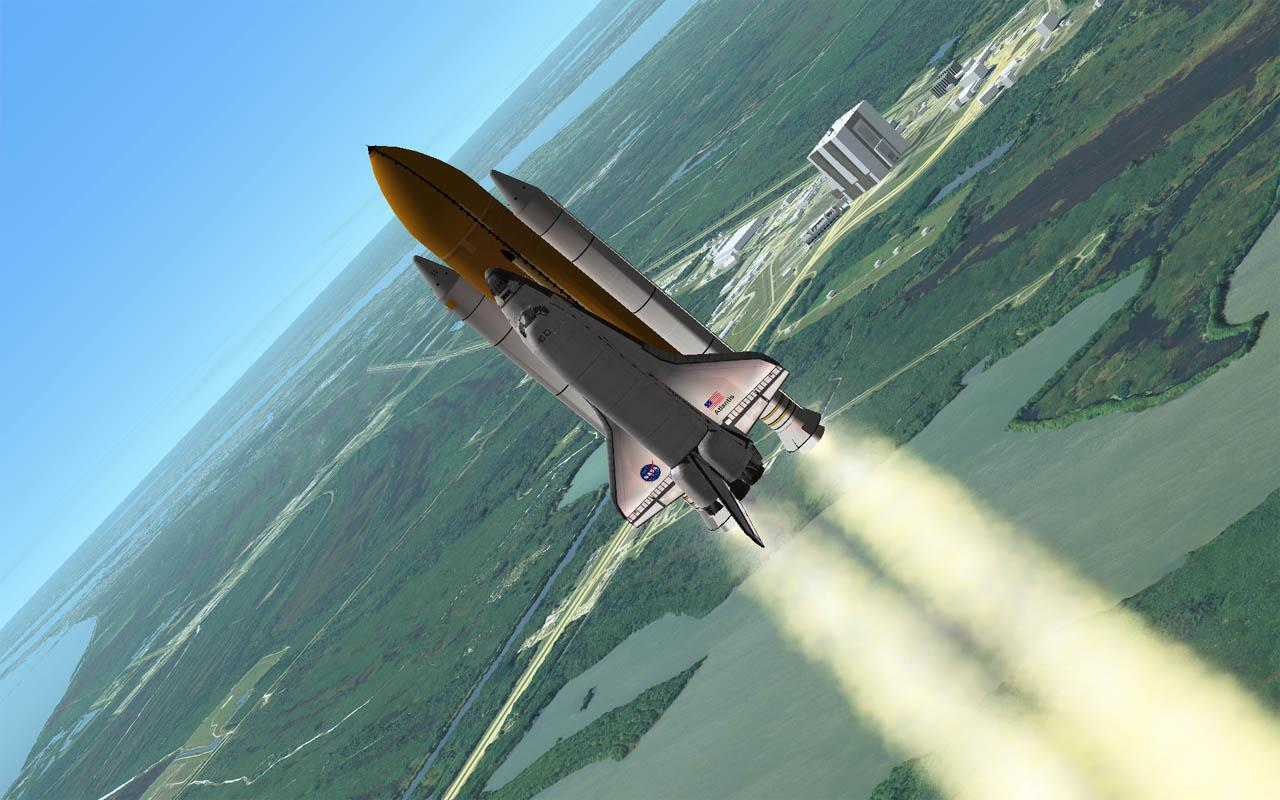
\includegraphics[width=0.99\hsize]{AtlantisLaunch.jpg}
\end{figure}

\textbf{Welcome to Orbiter 2016!}\\
\\
Orbiter 2016 is the latest instalment of the Orbiter Spaceflight simulator series. The most notable improvement from the 2010 Edition is the added support for surface elevation of planetary bodies, higher resolution surface and cloud textures, and improved surface collision modelling.\\
\\
High-resolution planetary texture packs are available for Earth, the Moon and Mars. In fact, there is now so much texture and elevation data available that you may need to free a bit of space on your hard disk to install it all – but I hope you'll agree that the result is worth the extra space.\\
\\
In addition, several of the spacecraft included in the standard distribution have had their cockpits updated and flight models improved. The simulation engine has been extensively reworked for improved stability.\\
\\
If the built-in graphics engine is not sufficient, Orbiter's interface for external graphics support has been extended. Try the excellent \textit{D3D9 Client} by Jarmo Nikkanen for advanced visual features and improved frame rates.\\
\\
As usual, the new version adds numerous bug fixes and feature enancements. Give it a try!\\
\\
\\
\textit{Martin Schweiger}

\end{document}
